\documentclass[a4paper]{article}
\usepackage[utf8]{inputenc}
\usepackage[catalan]{babel}
\usepackage{amsmath}
\usepackage{amsfonts}
\usepackage{amssymb}
\usepackage{graphicx}
\author{Joan Puigcerver Pérez}
\title{Títol del PFC}
\begin{document}
\maketitle

El reconeixement de text manuscrit (HTR) és una aplicació paradigmàtica del reconeixement de formes. En particular, el reconeixement de text manuscrit offline és una aplicació de gran interés ja que pot ser utilitzat, per exemple, per a transcriure el text en llibres i manuscrits antics per tal de preservar la informació o facilitar la cerca del seu contingut. \\

El principal problema del reconeixement de text manuscrit front a altres tasques de reconeixement és la variabilitat que es troba en la senyal d'entrada (en el cas del reconeixement offline, imatges que contenen text digitalitzat). Per exemple, un mateix autor no escriu un símbol sempre de la mateixa manera, ni de la mateixa grandària i ni tan sols amb la mateixa orientació. Per això, un dels components fonamentals de qualsevol sistema de reconeixement de l'escriptura és la normalització d'aquesta senyal d'entrada que tracta de reduir aquesta variabilitat. \\

Un pas que afecta a diferents parts de la normalització de la senyal és la detecció de les línies ascendents i descendents de la imatge (veure figura \ref{fig:adlines}). Diferents sistemes utilitzen diferents tècniques per a detectar aquestes línies. L'objectiu d'aquest projecte és el de comparar i quantificar les diferències entre dues d'aquestes tècniques, una basada en un enfocament heurístic \cite{Pastor07} i una altra basada en tècniques d'aprenentatge supervisat \cite{Espana10}. Les tècniques d'aprenentatge supervisat ofereixen un millor adjustament a la imatge, però el principal inconvenient és que requereixen la intervenció d'un humà durant l'entrenament de l'eina. El resultat d'aquest projecte ajudarà a prendre la decisió d'actualitzar l'eina de detecció de linies ascendents i descendents en un sistema que actualment utilitza la tècnica heurística, proveïnt als responsables amb dades dels beneficis obtinguts a l'utilitzar les tècniques d'aprenentatge supervisat.

\begin{figure}
\label{fig:adlines}
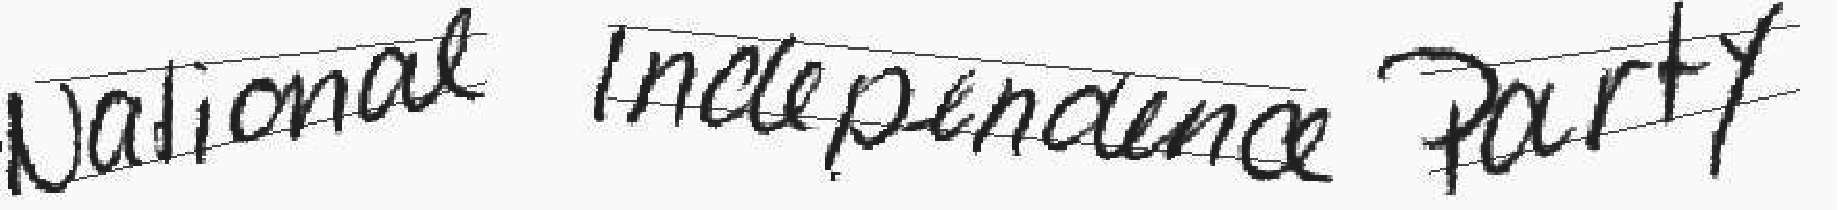
\includegraphics[width=\textwidth]{a01-011x-01_final}
\caption{Línies ascendents i descendents en una línia de text.}
\end{figure}

\begin{thebibliography}{9}
\bibitem{Pastor07} M. Pastor. \emph{Aportaciones al Reconocimiento Automático de Texto Manuscrito}. Ph.D. Thesis. 2007.

\bibitem{Espana10} S.Espana-Boquera, M.J.Castro-Bleda, J.Gorbe-Moya,F.Zamora-Martínez. \emph{Improving Offline Handwritten Text Recognition with Hybrid HMM/ANN Models}. IEEE Transactions on Pattern Analysis and Machine Intelligence. vol. 99. 2010.
\end{thebibliography}

\end{document}